\documentclass[12pt]{article}
\usepackage{hyperref}
\usepackage[letterpaper,left=1in,right=1in,top=1in,bottom=1in]{geometry}
\usepackage{setspace}
\usepackage{graphicx}
\usepackage{float}
\usepackage{listings}
\doublespacing
\usepackage{amsmath}
\lstset{
  basicstyle=\ttfamily,
  frame=single,
  breaklines=true,
}
\newcommand{\ignore}[1]{}
% im using the ubuntu package: "pdflatex" to compile this cause when I put pngs in it, that makes it easier
% hopefully that works for how you compile .tex files
\begin{document}
~\\
Scott Griffy \\
Robert Handy \\
Spring 2019 \\
CS545 - Machine Learning \\
Teacher: Anthony Rhodes \\
Assignment: Final Project Write-Up \\
Presented: June 10th, 2019 \\
\par
The EMBER dataset is a set of binaries.
The white paper can be found at: \url{https://arxiv.org/abs/1804.04637} and the code used to manipulate the dataset can be found at \url{https://github.com/endgameinc/ember}.
The dataset is designed to assist with training malware classifiers using machine learning to classify malicious binaries.
The dataset consists of a training set of 300K malware binaries, 300K benign binaries (binaries that do not have an adverse affect on computers), 300K unlabeled binaries (these could be either malicious or benign, it is not known which).
The dataset also includes a test set consisting of 100K malicious binaries and 100K benign binaries.
\par
Finding data to use for machine learning models that classify malware is a difficult task.
One of the problems in acquiring and publishing a dataset is licensing issues surrounding the binaries in the dataset.
Many binaries are not permitted for distribution because of commercial licenses.
The authors of the EMBER dataset avoided this by releasing features of binaries in place of the actual binaries.
\par
The authors of EMBER removed the actual binaries from this dataset.
This protects the researchers performing the machine learning algorithms.
If malicious binaries were included in the dataset, the researchers could potentially infect themselves while training a model.
\par
Another large contribution of the authors of the EMBER dataset is the labels of the binaries. Labeling binaries is difficult work, which is generally done by hand by experts. Because of this difficultly and level of skill required, a label indicating binaries as malware or benign is very valuable. This dataset contains 800K labeled features of binaries.
\par
In our project, we used this dataset to train different machine learning models.
We used a Bayesian learning algorithm on the labeled data of the EMBER dataset, and a K-means algorithm on the unlabeled data.
\section{K-Means}
\par
The unlabeled data in the dataset is meant to be used for semi-supervised learning.
This was out of scope for this project as we did not learn about semi-supervised techniques in class.
Hopefully the unsupervised model we performed on the data (and the model's analysis) is interesting enough to be a significant contribution to understanding how the EMBER dataset can be used for machine learning models.
\par
We used the k-means algorithm to do unsupervised learning. A PCA dimensionality reduction was run on the data to reduce the features from 2351 to 2. This allows us to graph the data points in 2-D space.
The problem with running a fully unsupervised scheme rather than using a semi-supervised algorithm is that the unsupervised algorithm may find a different distinction than malicious or benign.
The k-means ended up getting 50\% accuracy on the test data, which, because the test data was evenly split, was just as good as guessing.
After graphing the points retrieved from PCA and categorized with k-means it seemed that the k-means algorithm had strictly split the data along the x-axis.
After graphing the test points and their classifications, we noticed that the y-axis actually did a much better job of separating the data.
Just using the y-axis as a classifier, and choosing a split based on the average y value of training points, we achieved an accuracy of 70\%.
Here's an example run of the program:
\begin{lstlisting}
$ python3 kmeans/kmeans.py 10000 5000
original # dimensions 2351
# unlabeled 10000
# pos 2500
# neg 2500
scaling...
pca-ing to  2  dimensions...
max args: - pca component vectors (out of 2351 features)
         1473
         509
training (kmeans on 2 centers)...
FOR DEBUGGING:
         label min 0
         label max 1
testing...
total 5000
correct 2557.0
accuracy 0.5114
confusion_matrix
 [[2426.   74.]
 [2369.  131.]]
totalEntropy - kmeans 0.8136407057087205

==Classifying using minor axis in 2 dim PCA==
meany 2.3874235921539365e-16
totalEntropy - pca1 0.7617772608209377
y eval (# correct,total) 3511 5000
y eval accuracy 0.7022
creating graphs
saving learning cluster to  ./kmeans_clusters.png
saving guess cluster to  ./kmeans_guesses.png
\end{lstlisting}

\begin{figure}[H]
\centering
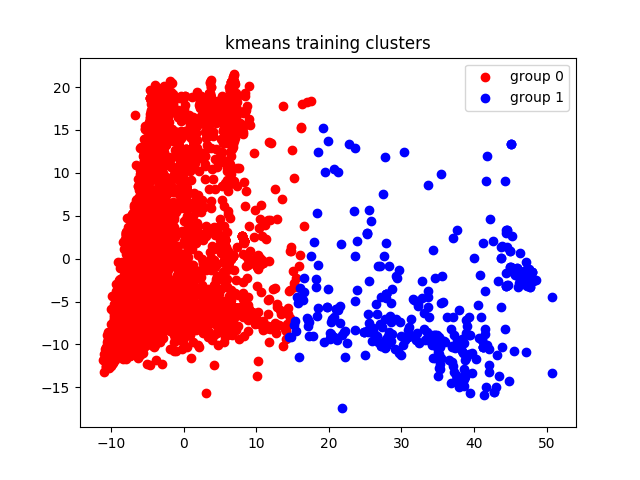
\includegraphics[width=.5\textheight]{kmeans_clusters}
\end{figure}
\begin{figure}[H]
\centering
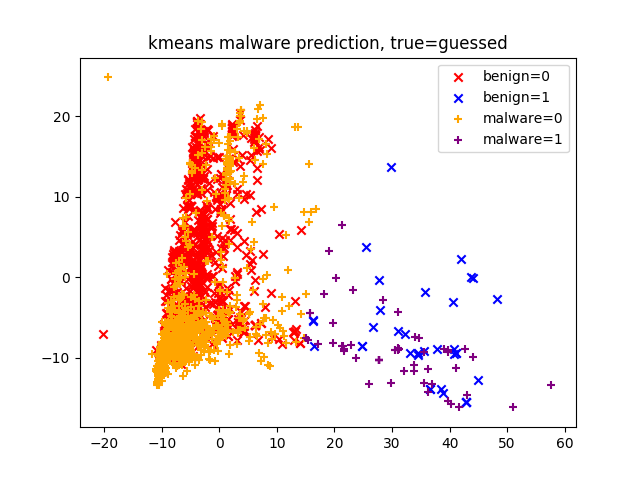
\includegraphics[width=.5\textheight]{kmeans_guesses}
\end{figure}
\section{Bayesian}
\par
Your stuff here
\section{Conclusion}
\par
Write this later.
\end{document}
